\chapter{Lines and Planes}
\label{Chapter:03linesplanes}

In the last chapter we discussed the algebra and geometry of vectors in
$\R^2$ and $\R^3$, and extended all the notions of vector addition,
scalar multiplication, the dot product, angles and orthogonality
to $\R^n$.  

Now, let's consider lines and planes in $\R^2$ and $\R^3$.  
We'll see that while some ideas generalize easily
to $\R^n$, others take more work; in fact, working out what, exactly,
a reasonable analogue of a line or a plane in $\R^n$    
is one of our goals in this course.


\section{Describing Lines}

A line in $\R^2$ or $\R^3$ 
is completely determined by specifying its direction and
a point on the line.  Since we prefer working with vectors, replace
the point by its position vector.

\begin{figure}
\begin{center}
\vglue-.7cm

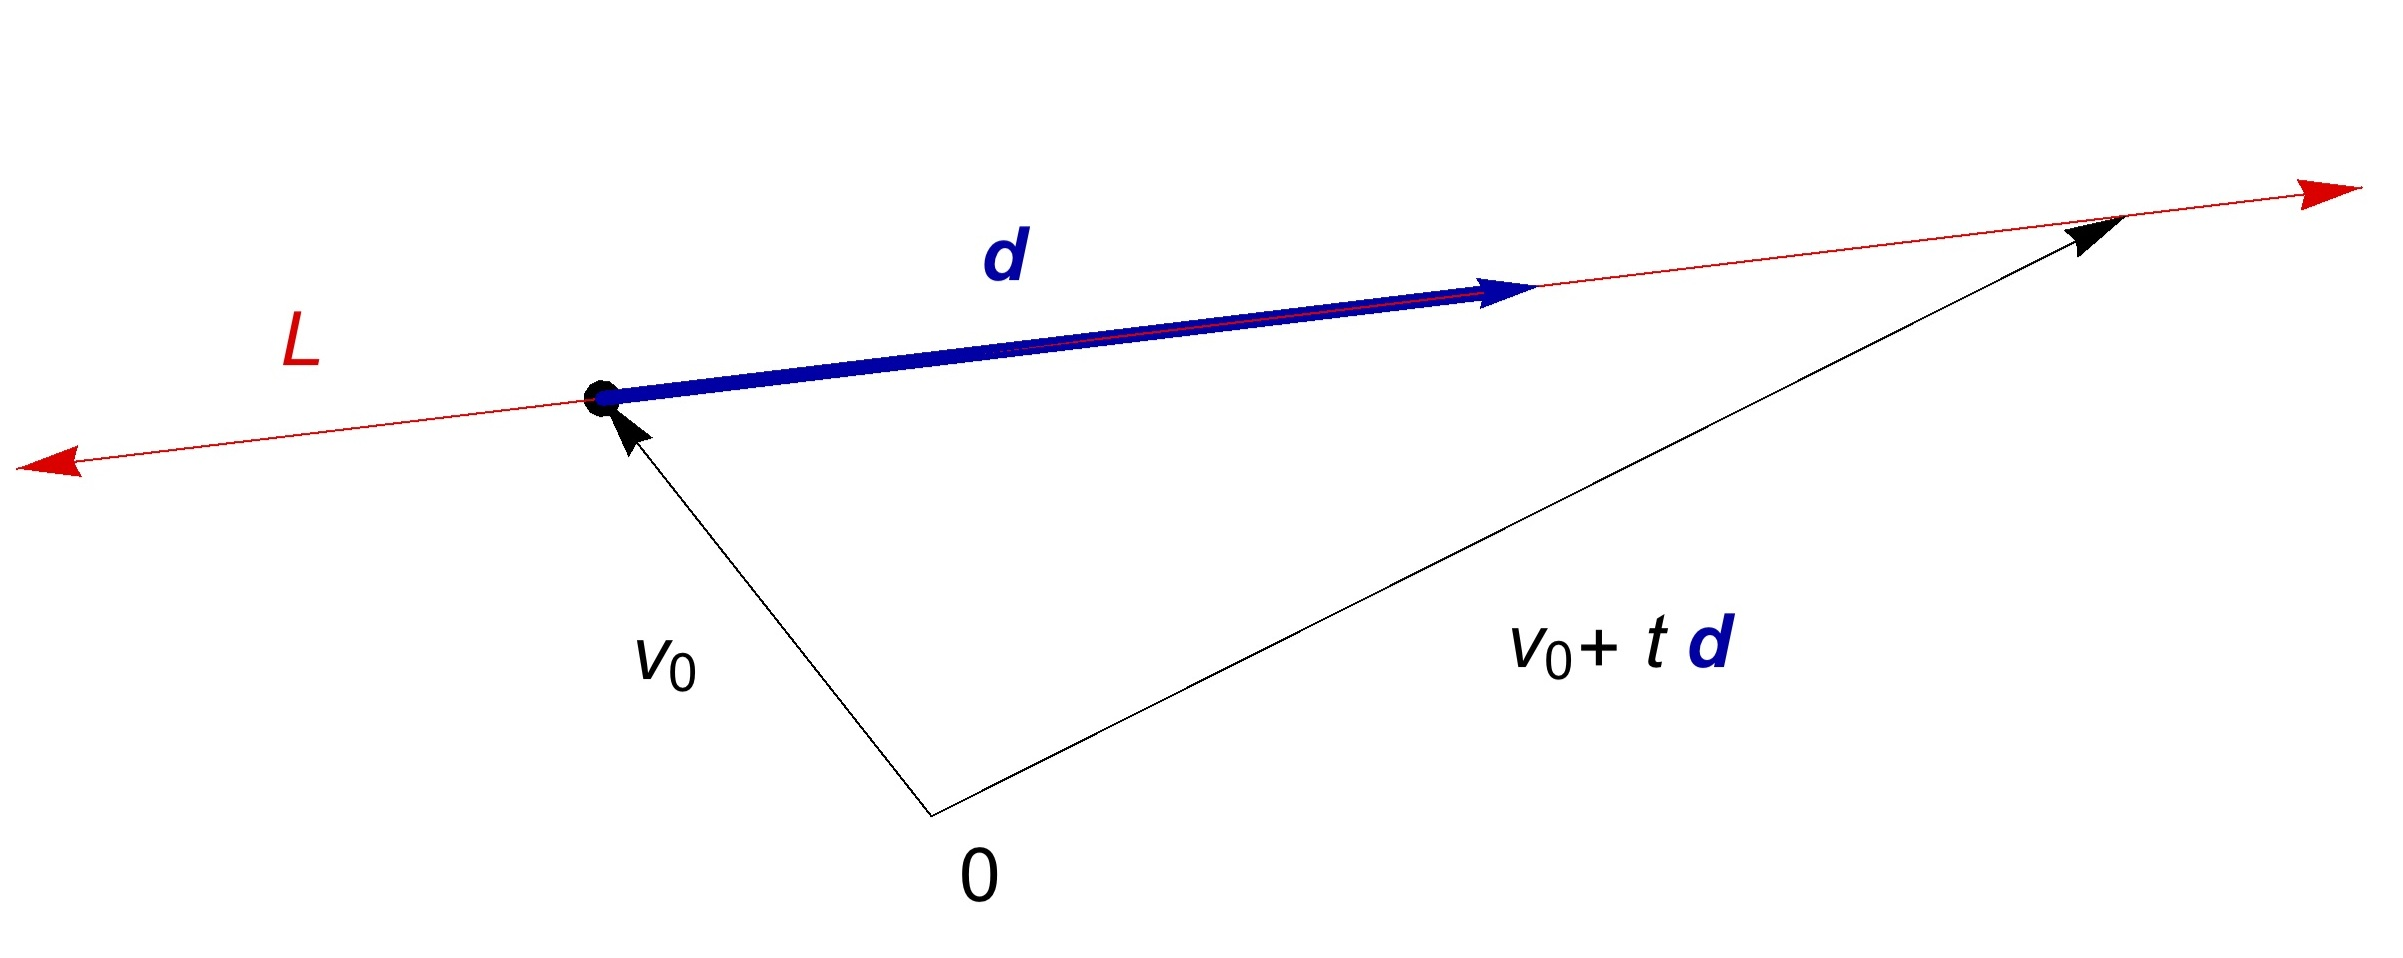
\includegraphics[scale=.1]{img/linepoint-directionvector.jpg}
\end{center}

\caption{Vector parametric form for $L$}\label{vectorparametricformplane}
\end{figure}


So a line $L$ going through the tip of $\vv_0$ and such that $\dd$
is a vector parallel to the direction of $L$ can be described as
the set
$$
L = \{ \vv_0 + t \dd | t\in \R\}.
$$
That is, any point $\vv$ on the line $L$ can be written as $\vv = \vv_0+t\dd$ for some $t$.

\begin{myexample}
Consider the line $y=3x+2$ in $\R^2$.  We can get a parametric equation for
this line by letting $x=t$ be the parameter and solving for $y$; this gives
$x = t$ and $y=3t+2$.  In vector form, this is
$$
\mat{x\\y} = \mat{t\\3t+2} = \mat{0+1t\\2+3t} = \mat{0\\2} + t\mat{1\\3}
$$
so the line is
$$
L = \left\{ \mat{0\\2} + t\mat{1\\3} \Big| \, t \in \R\right\}.
$$


Note:  Another way to get a parametric equation for this line:  it
 goes through the points $(0,2)$ and $(-\frac{2}{3},0)$,
for example.  So a direction vector is
$$\dd = \mat{0\\2}-\mat{-2/3\\0} = \mat{2/3\\2}.$$
We can take $\vv_0 = (0,2)$.  So we get
$$
L = \left\{ \mat{0\\2} + t\mat{2/3\\2} \Big|\, t\in\R\right\}.
$$
NOTICE  that our answer is not unique!  It depends on our choices.
BOTH of our answers are completely correct (check with a sketch!).
\end{myexample}

CAUTION!!  We often use the variable $t$ for the parameter.  But if
you are comparing two different lines, you must use different
letters to represent parameters on different lines!

\begin{myexample}
Find the point of intersection of $L = \{ t(1,2) | t \in \R\}$
and $L' = \{ (0,1)+t(3,0) | t \in \R\}$.

WRONG METHOD: Set $t(1,2)=(0,1)+t(3,0)$ and solve for $t$.

This doesn't give an answer for $t$; but that's only because
the two lines don't arrive at the point of intersection at
the same time $t$.  The lines still intersect!

CORRECT METHOD:  Find parameters $s$ and $t$ such that
 $t(1,2) = (0,1)+s(3,0)$.  This gives $t=\frac12$ and $s=\frac16$,
and the point of intersection is thus $(\frac12,1)$.
\end{myexample}

The form
$$
L = \{ \vv_0 + t \dd | t\in \R\}
$$
for a line in $\R^n$ is called the \defn{vector form} or \defn{parametric 
form}.  In $\R^2$ (but NOT $\R^3$), you can describe a line by an equation like
$ax+by=c$; this is called the \defn{point-normal} or \defn{Cartesian form}.

You can also expand the parametric form in coordinates:  if $\vv_0 = (a,b,c)$ and $\dd = (d_1,d_2,d_3)$ then our line
is the set of all $\vv=(x_1,x_2,x_3)$ such that 
\begin{align*}
x_1 &= a+ td_1\\
x_2 &= b+td_2\\
x_3 &= c+td_3
\end{align*}
for some $t\in \R$.

\section{About the Geometry of Lines}

There is only one line in $\R$:  all of $\R$.

Given two distinct lines in $\R^2$, they are either parallel or they intersect.

Given two distinct 
lines in $\R^3$, they could be parallel, or they could intersect,
or they could be skew.  In the first two cases, they are contained
in a unique plane; in the third case there is no plane containing
both of them (but you can find two parallel planes such that each
contains one of the lines).

\section{Describing Planes in \texorpdfstring{$\R^3$}{R3}}
Recall that planes in $\R^3$ are described by an equation in point-normal
 or  Cartesian form.  That is, a plane is described as 
the set of all points $(x,y,z)$ such that
$$
ax+by+cz = d
$$
where $\nn = (a,b,c)$ is a \emph{normal vector} to the plane
and $d\in \R$.

How did we get this equation? Look below. If $\vv_0$ is some point on the plane, then $\vv$ is on the plane iff $(\vv - \vv_0) \cdot \nn = 0$:  \begin{figure}
\begin{center}
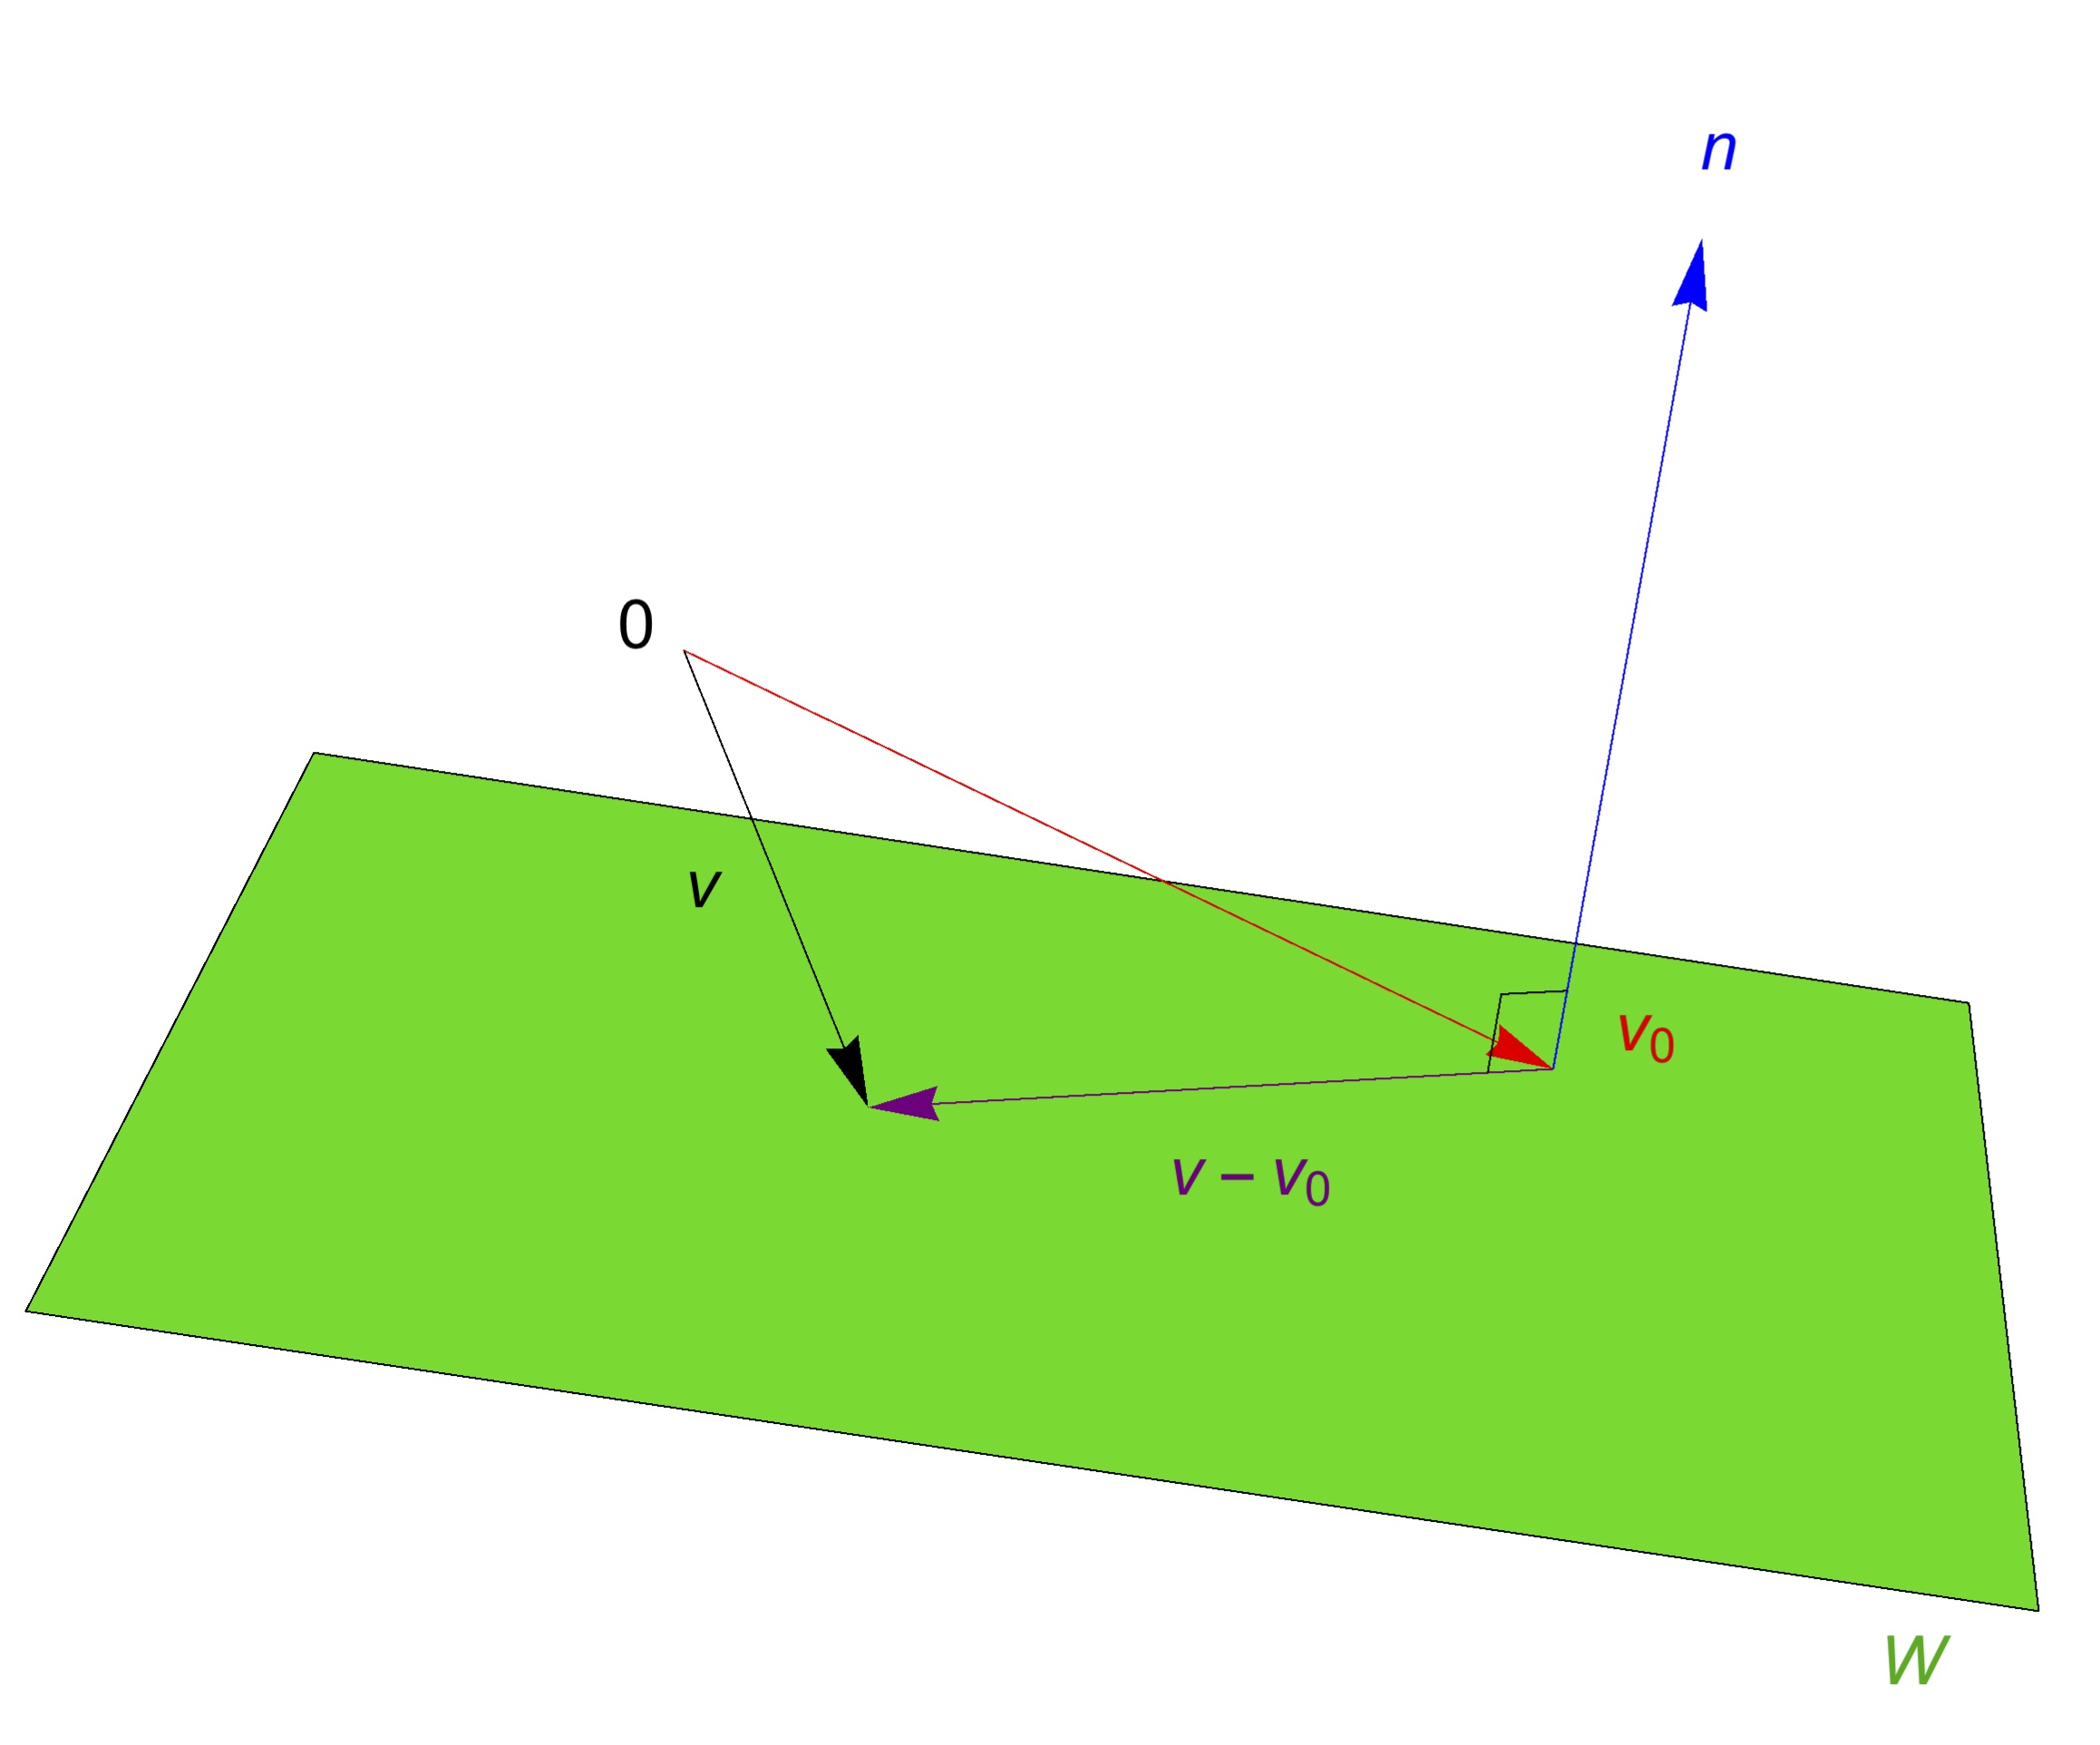
\includegraphics[width=4in]{img/cartesianequationplane.jpg}
\end{center}

\caption{The cartesian equation of a plane: point-normal form}\label{cartesiannormalformplane}
\end{figure}

So the plane through $\vv_0$ with normal vector $\nn$ is
$$
W = \{ \vv \in \R^3 | (\vv - \vv_0) \cdot \nn = 0 \}.
$$

\begin{myexample}
The plane through $\vv_0 = (1,0,3)$ with normal vector $\nn = (-1,1,2)$
is
\begin{align*}
W &= \{ \vv \in \R^3 | (\vv-\vv_0)\cdot \nn=0\}\\
&= \{ (x,y,z) | ((x,y,z)-(1,0,3))\cdot (-1,1,2)=0\}\\
&= \{ (x,y,z) | -(x-1)+(y-0) + 2(z-3) = 0\}\\
&= \{ (x,y,z) | -x+y+2z = 5\}
\end{align*}
(Note that the coefficients in the Cartesian equation give you a normal vector.)
\end{myexample}

The normal vector is handy for many things.

\begin{myprob} 
Find the distance from the point $P = (1,2,3)$
to the plane $W$ with Cartesian equation $3x-4z=-1$.

\begin{mysol} 
%\begin{figure}



%\end{figure}
Let $A$ be any point on the plane, say $A=(1,0,1)$, and $Q$ be the (unknown) closest point on the plane to $P$.
As the diagram suggests\footnote{And here's a proof, for the properly skeptical reader: if $Q'$ is any other point on $W$, $\|P-Q'\|^2=\|P-Q+ Q-Q'\|^2= \|P-Q\|^2+ \|Q-Q'\|^2$ (because $P-Q$ and $Q-Q'$ are perpendicular, so the Pythagorean theorem applies). Hence $\|P-Q'\|^2\ge  \|P-Q\|^2$. }, we want the length of the projection of $A-P$ onto the normal vector.

\begin{center}


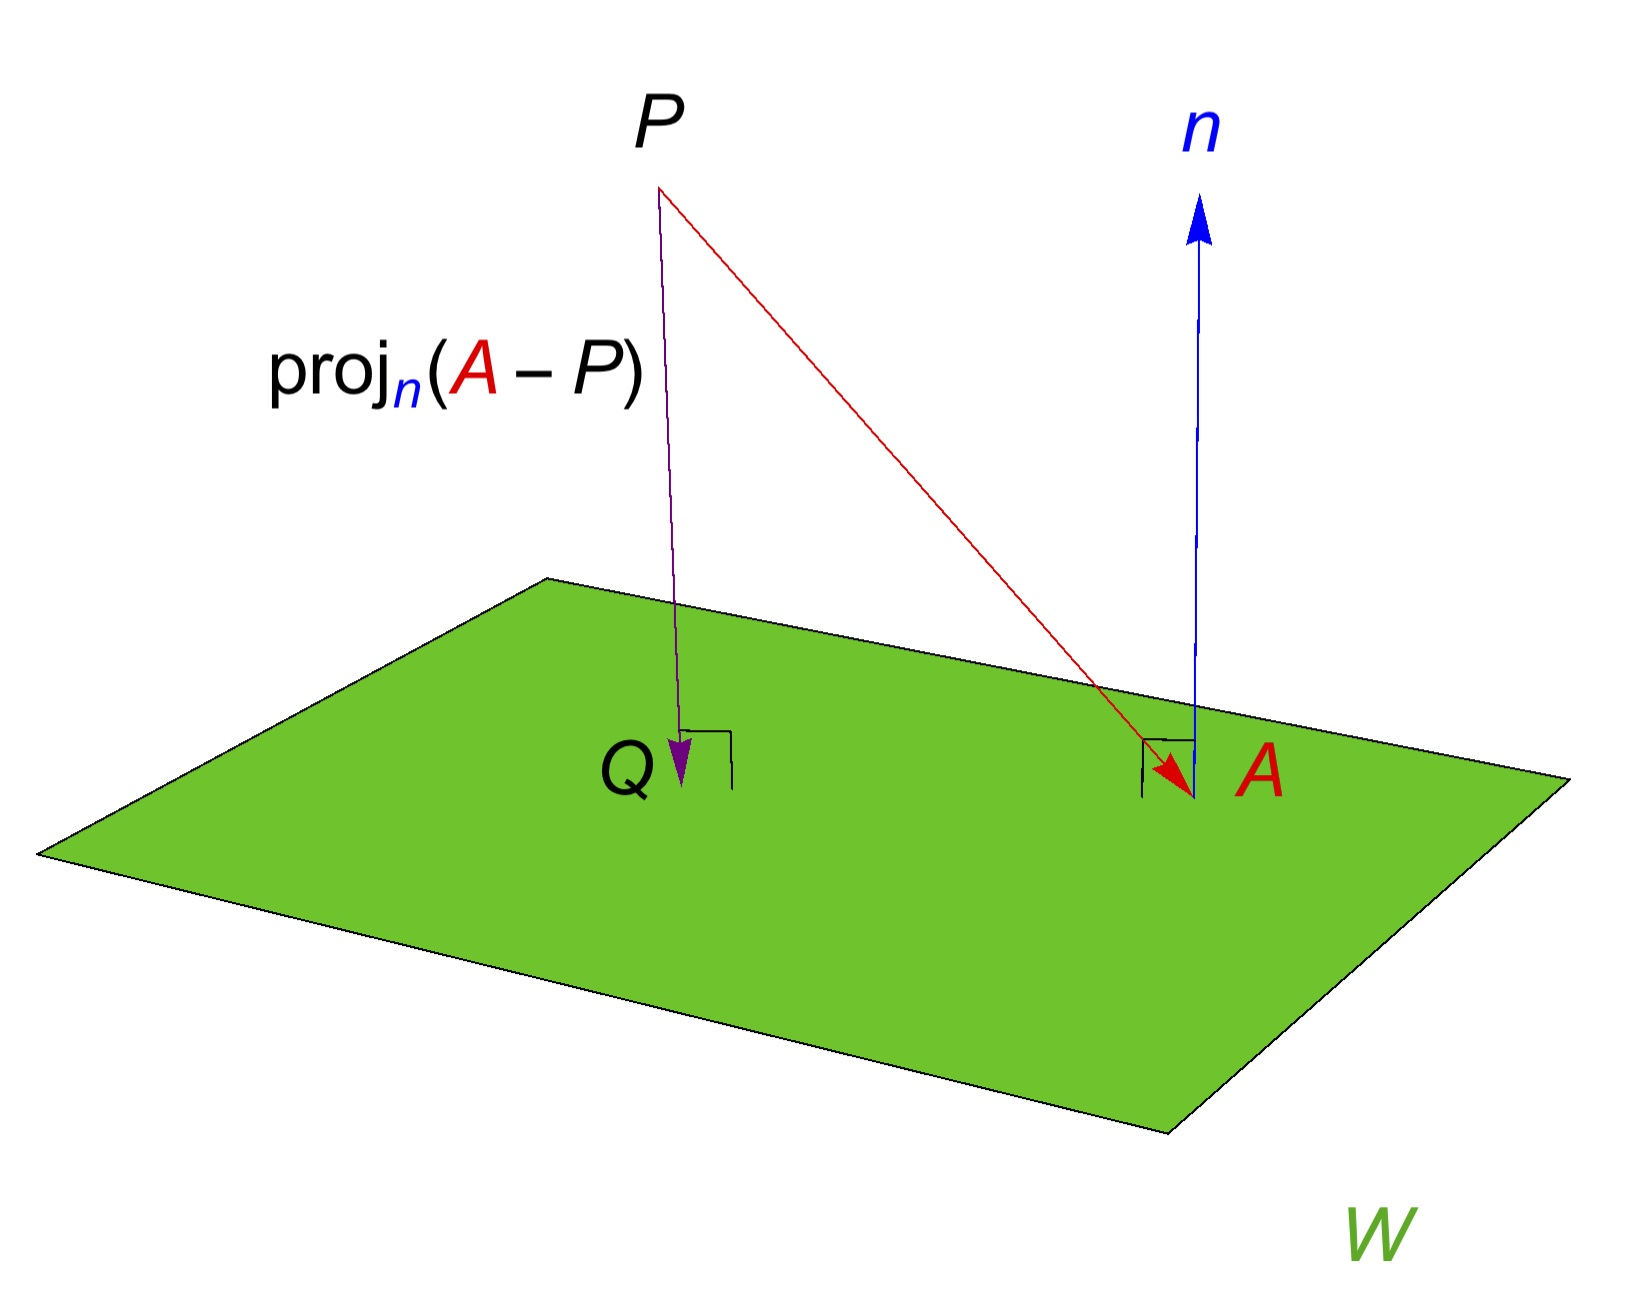
\includegraphics[scale=.5] {img/projP_on_W.jpg}

{Finding the distance of P to the plane $W$.} 
\end{center}


So
\begin{align*}
\Vert P-Q \Vert &= \Vert {\proj}_{\nn}(P-A) \Vert\\
&= \Vert {\proj}_{(3,0,-4)}(0,2,2) \Vert\\
&= \Vert \frac{0+0-8}{3^2+(-4)^2}(3,0,-4) \Vert\\
&= \frac{8}{25} \Vert (3,0,-4) \Vert\\
&= \frac{8}{25} \sqrt{25} = \frac{8}{5}.
\end{align*}
\end{mysol}
\end{myprob}

Let's tackle a more straightforward problem: the intersection of
two planes.

\begin{myprob} Find the intersection of the planes $x+y+z = 3$ and $x-y-z=2$.

\begin{mysol} We need to find all $(x,y,z)$ which satisfy both equations.
Subtracting the second equation from the first yields $2y+2z = 1$
or $y = \frac12-z$; then from the first we have $x = 3-(\frac12-z)-z
= \frac52$.  But $z$ can be anything; in fact we can take
$z$ to our parameter (and so now call it $t$):
$$
x = \frac52, \quad y=\frac12-t, \quad z=t
$$
which in vector form is the line
$$
L= \left\{ \mat{5/2\\1/2\\0} + t \mat{0\\-1\\1} | t\in \R\right\}.
$$
\end{mysol}\end{myprob}

\section{Geometry of Planes in \texorpdfstring{$\R^3$}{R3}}

We define the ``angle'' between two planes to
be the angle between their normal vectors.  It equals
the angle of the ``wedge'' that they make (although
proving that takes some thought).

Now, to compare with the case of lines:
 
The only plane in $\R^2$ is all of $\R^2$.

Given two distinct planes in $\R^3$, they are either parallel
or they intersect.

Makes you wonder about $\R^4$, doesn't it?

That said, we don't have a good way to describe a plane in $\R^4$
(yet).  
A parametric equation in one variable gives a line, in any
$\R^n$.  But something fishy is happening with the normal
forms:

\begin{center}
\begin{tabular}{cccc}
$n$ & & Equation in $\R^n$& Resulting Geometric Object \\
\hline
1 &\hphantom{XX} & $ax=b$ & point \\
2 & & $ax+by=c$ & line \\
3 & & $ax+by+cz =d$ & plane\\
4 & & $ax_1+bx_2+cx_3+dx_4=e$ & ??
\end{tabular}
\end{center}

Idea:  one equation is cutting down one \stress{degree of freedom}
(later: \defn{dimension}), so the result is always an object
of \stress{dimension $n-1$} (which is called a \defn{hyperplane} in dimensions bigger than 3).

Our answer will eventually be:  Since intersecting two planes in $\R^3$
(usually) gives you a line, intersecting two hyperplanes in $\R^4$ should
give you a plane.


This is something we'll be coming back to over the next
few weeks.


But for now: let's get back to solid ground (or rather, $\R^3$) and
discuss how to produce normal vectors to planes fairly easily.

\section{Cross products in \texorpdfstring{$\R^3$}{R3}}


Let's use the notation:
$$
\hat{i} = \mat{1\\0\\0}, \quad \hat{j} = \mat{0\\1\\0}, \quad \hat{k} = \mat{0\\0\\1}.
$$
Then $(x,y,z) = x\hat{i} + y\hat{j} + z\hat{k}$.

In the following, we also use notation from the \emph{determinant}
which for now is just very convenient.

The \defn{cross product} of $\uu = (x,y,z)$ and $\vv=(x', y', z')$
is a new vector, denoted $\uu \times \vv$, which is calculated 
as follows:
\begin{align*}
\uu \times \vv &= \left| \begin{matrix}
\hat{i} & \hat{j} & \hat{k} \\
x & y & z\\
x' & y' & z' \end{matrix} \right|\\
&= \left( yz' - y'z, -(xz' - x'z), xy' - x'y \right) \\
&= \left( \left| \begin{matrix} y & z\\ y' & z' \end{matrix} \right|,
- \left| \begin{matrix} x & z\\ x' & z' \end{matrix} \right|,
\left| \begin{matrix} x & y\\ x' & y' \end{matrix} \right| \right)
\end{align*}

\begin{myprob}
Find $(1,2,3)\times(4,5,6)$.

\begin{mysol}  Write this as a determinant (or at least on top of each other)
and then solve:
$$
\left| \begin{matrix}
\hat{i} & \hat{j} & \hat{k} \\
1 & 2 & 3\\
4 & 5 & 6 \end{matrix} \right|
= (12-15, -(6-12), 5-8) = (-3,6,-3). 
$$
\end{mysol}\end{myprob}

\begin{myprob} Find $(4,5,6)\times(1,2,3)$.

\begin{mysol} Same process:
$$
\left| \begin{matrix}
\hat{i} & \hat{j} & \hat{k} \\
4 & 5 & 6\\
1 & 2 & 3 \end{matrix} \right|
= (15-12, -(12-6), 8-5) = (3,-6,3)
$$
HA!  We got the NEGATIVE. 
\end{mysol}\end{myprob}

Notice, though, that
$$
(1,2,3)\cdot (3,-6,3) = 3-12+9 = 0, \quad (4,5,6)\cdot (3,-6,3) = 12-30+18=0.
$$
None of this was just luck.

\begin{theorem}[Properties of the Cross Product]
Let $\uu,\vv,\ww\in \R^3$.  Then
\begin{itemize}
\item $\uu \times \vv = -\vv \times \uu$
\item $(\uu \times \vv)\cdot \uu = 0$
\item $(\uu \times \vv)\cdot \vv = 0$
\item $(\uu + \vv)\times \ww = \uu \times \ww + \vv \times \ww$
\item $\Vert \uu \times \vv \Vert = \Vert \uu \Vert \; \Vert \vv \Vert \sin(\theta)$ where $0 \leq \theta \leq \pi$ is the angle between $\uu$ and $\vv$.
This is in fact the area of the parallelogram with sides $\uu$ and $\vv$.
\end{itemize}
BUT, usually:  $\uu \times (\vv \times \ww) \neq (\uu \times \vv) \times \ww$;
the cross product is neither commutative nor associative.  (Eg:  $\hat{i} \times (\hat{k} \times \hat{k}) = \zero$ but $(\hat{i} \times \hat{k})\times \hat{k} = -\hat{i}$.)
\end{theorem}


Consequently:
if two vectors are parallel, then their cross product
is zero.  Otherwise, their cross product is one of the two vectors orthogonal to both 
$\uu$ and $\vv$ and of length $\Vert \uu \Vert \; \Vert \vv \Vert \sin\theta$, where $\theta$ is the angle between $\uu$ and $\vv$.
The cross product is used in Physics for measuring torque, for example,
and figuring out the direction of the answer uses the
right-hand rule.  We also often memorize $\hat{i} \times \hat{j} = \hat{k}$ and its cyclic permutations.

\section{First application of cross product: finding normal vectors}

The cross product gives a normal vector to the plane parallel to two vectors $\uu$ and $\vv$.

\begin{myprob}
Find an equation of the plane containing the three points $A = (1,2,3)$,
$B = (1,0,0)$ and $C = (0,1,1)$.

\begin{mysol}
The vectors $\vec{BA} = (0,2,3)$ and $\vec{BC} = (-1,1,1)$ are both
parallel to the plane, so a normal vector to the plane must be
orthogonal to each of these.  So take their cross product:
$$
 \left| \begin{matrix}
\hat{i} & \hat{j} & \hat{k} \\
0 & 2 & 3\\
-1 & 1 & 1 \end{matrix} \right| = (-1, -3, 2)
$$
(Check your answer!  This should be orthogonal to $\vec{BA}$
and $\vec{BC}$.)

So an equation for the plane has the form
$$
-x -3y + 2z = d
$$
and plugging in the point $B$, for example, yields $d=-1$.
\end{mysol}\end{myprob}

\section{Second Application:  volumes of parallelepipeds (Scalar Triple Product)}

\begin{theorem}[Volume of a parallelepiped]
The volume of the parallelepiped with sides $\uu$, $\vv$ and $\ww$
in $\R^3$ is
$$
\vert (\uu \times \vv) \cdot \ww \vert. 
$$
In particular, the order of the vectors doesn't matter.
\end{theorem}

We can prove this using more trigonometry:  the volume of
the parallelepiped is the area of the base (a parallelogram)
times the height; the area of the base is the norm of the cross product
of two of the vectors ($\Vert \uu \times \vv \Vert$), and the height is going to be 
$\Vert \ww \Vert \cos(\theta)$ where $\theta$ is the angle between
$\ww$ and a normal vector to the base.

\begin{myprob}
Find the volume of the parallelepiped with sides $\uu = (1,0,1)$,
$\vv = (1,2,2)$ and $\ww = (10,0,0)$.

\begin{mysol}
We calculate:
$$
\uu \times \vv =  \left| \begin{matrix}
\hat{i} & \hat{j} & \hat{k} \\
1 & 0 & 1\\
1 & 2 & 2 \end{matrix} \right| 
= (-2,-1,2)
$$
so
$$
(\uu \times \vv)\cdot \ww = (-2,-1,2)\cdot (10,0,0) = -20
$$
so the volume is $20$.
\end{mysol}\end{myprob}

So what does it mean if $(\uu \times \vv)\cdot \ww = 0$?  Zero
volume of a parallelepiped means it wasn't really a parallelepiped
at all --- the three vectors must all lie in a plane.  We
say such vectors are \defn{coplanar} or \defn{linearly dependent}
(key phrase for later).





\section{Final remarks about lines, planes, and higher-dimensional
objects in \texorpdfstring{$\R^n$}{Rn}}  

These are just some thoughts to preview some of the ideas
we want to explore over the next several weeks.  We have
great ways to describe lines and planes in $\R^2$ and $\R^3$,
but we have an inkling that there must be ``2-dimensional'' objects
in $\R^4$ which we can't describe by either of the two
methods described so far (parametric equations or normal equations).

Or can we?  

To get a line,
we gave ourselves one parameter (one degree of freedom).  If
we give ourselves two parameters, for two different direction
vectors, this describes a plane.  That is
$$
W = \{ \vv_0 + s\dd_1 + t\dd_2 | s,t\in\R\}
$$
describes the plane with normal vector $\dd_1 \times \dd_2$
and going through the point $\vv_0$.

We will explore statements like this in the course of understanding
subspaces of general vector spaces.



